\documentclass[UTF8,a4paper,12pt]{ctexart}

\usepackage{amsmath,amssymb}
\usepackage{booktabs}
\usepackage{caption}
\usepackage{float}
\usepackage{geometry}
\usepackage{graphicx}
\usepackage{hyperref}
\usepackage{longtable}
\usepackage{xcolor}
\usepackage{enumitem}
\usepackage{fvextra}

\geometry{left=2.6cm,right=2.6cm,top=2.6cm,bottom=2.6cm}
\hypersetup{colorlinks=true,linkcolor=black,urlcolor=blue}
\setlength{\parindent}{2em}
\setlength{\parskip}{0.25em}
\setlength{\emergencystretch}{3em}
\sloppy
\linespread{1.25}
\setlist[itemize]{leftmargin=2.5em,itemsep=0.15em}
\DefineVerbatimEnvironment{CodeBlock}{Verbatim}{breaklines,breakanywhere,fontsize=\small,frame=single,rulecolor=\color{gray!45}}

\title{\heiti 机器学习与Python实践\\[0.8em]\Large 第四次作业\\[1.6em]\Huge 基于学习行为数据的学生成绩等级分类模型}
\author{}
\date{}

\begin{document}

\begin{titlepage}
    \centering
    \vspace*{1.2cm}
    
\includegraphics[width=0.78\linewidth]{figures/cover_logo.png}\par
    \vspace{1.0cm}
    {\zihao{2}\heiti 机器学习与Python实践\par}
    \vspace{0.8cm}
    {\zihao{3}\heiti 第四次作业\par}
    \vspace{1.2cm}
    {\zihao{1}\heiti 基于学习行为数据的学生成绩等级分类模型\par}
    \vfill
    \begin{tabular}{rl}
        姓名：& 匿名\\[0.45em]
        专业：& 强基班\\[0.45em]
        学号：& \\[0.45em]
        教师：& 匿名\\[0.45em]
        学院：& 信息科学与工程学院\\[0.45em]
    \end{tabular}
    \vfill
    {\zihao{4}2026年6月5日\par}
\end{titlepage}

\tableofcontents
\newpage

\section{前言及问题概述}

随着在线学习平台和移动端学习管理系统的发展，学生在学习过程中的行为数据能够被较为完整地记录下来。例如，上课举手次数、访问课程资源次数、查看课程公告次数、参与讨论次数、家长是否参与问卷、缺勤情况等信息，都可以从不同角度反映学生的学习投入程度和外部支持情况。若能利用这些数据对学生成绩等级进行预测，就可以帮助教师更早发现潜在风险学生，并为教学干预、家校沟通和学习资源推送提供参考。

本次实验使用题目给出的 \texttt{kalboard360\_xAPI\_Edu\_Data.csv} 数据集。该数据来自手机 APP ``Kalboard 360'' 的学习管理系统，平台旨在利用云端技术提升 K-12 教育中的学习管理水平。数据集共包含 480 条学生记录和 16 个输入特征，目标变量为 \texttt{Class}，表示学生成绩等级，取值包括 \texttt{L}、\texttt{M} 和 \texttt{H}，分别代表低、中、高三个等级。

题目要求是根据学习者在学习活动中的特征预测学生成绩等级。因此，本实验属于监督学习中的多分类问题。实验过程包括数据读取、数据预览、探索性分析、特征工程、类别编码、模型训练、模型评价和可视化展示。为了使结果更可靠，本文同时比较多数类基线、逻辑回归、支持向量机、随机森林和梯度提升等模型，并使用准确率、宏平均 F1 值、平衡准确率和混淆矩阵综合评价模型效果。

\section{相关基础知识及方法}

\subsection{相关原理}

分类任务的目标是根据输入特征向量 $x$ 判断样本所属类别 $y$。在本实验中，$x$ 表示一名学生的学习行为、人口统计和教育背景特征，$y\in\{L,M,H\}$ 表示学生成绩等级。分类模型可以表示为
\begin{equation}
    \hat{y}=f(x),
\end{equation}
其中 $\hat{y}$ 是模型预测的类别。模型训练的核心目标是从已有标注样本中学习类别边界，使模型在未见过的测试样本上仍能保持较好的判断能力。

逻辑回归是常用的线性分类模型。对于多分类任务，可以将二分类逻辑回归扩展为多项逻辑回归，模型输出每个类别的概率，并选择概率最高的类别作为预测结果。逻辑回归训练速度快、解释性较好，但其决策边界主要是线性的，对复杂非线性关系表达能力有限。

支持向量机通过寻找能够最大化类别间隔的分类超平面来完成分类。当使用 RBF 核函数时，支持向量机可以在高维特征空间中形成非线性分类边界，适合处理中小规模、类别边界较复杂的数据。随机森林则由多棵决策树集成而成，通过样本和特征的随机抽样降低过拟合风险；梯度提升模型同样基于决策树，但采用逐步拟合残差的方式不断提高模型表现。

由于本数据集的目标类别不是完全均衡，仅使用准确率可能会掩盖少数类别的预测问题。因此，本文重点使用宏平均 F1 值和平衡准确率。对于单个类别，精确率、召回率和 F1 值分别定义为
\begin{equation}
    Precision=\frac{TP}{TP+FP},
\end{equation}
\begin{equation}
    Recall=\frac{TP}{TP+FN},
\end{equation}
\begin{equation}
    F1=\frac{2\times Precision\times Recall}{Precision+Recall}.
\end{equation}
宏平均 F1 是对所有类别 F1 值直接取平均，因此每个类别的权重相同，更能反映模型对三类学生的整体识别能力。

\subsection{数据描述}

数据集文件为 \texttt{kalboard360\_xAPI\_Edu\_Data.csv}，读取后共有 480 行、17 列，其中 16 列为输入特征，1 列为目标变量。数据中没有缺失值，因此不需要进行额外缺失值填补。主要字段含义见表 \ref{tab:features}。

\begin{longtable}{lll}
\caption{Kalboard 360 学生成绩等级数据集字段说明}\label{tab:features}\\
\toprule
字段 & 类型 & 含义\\
\midrule
\endfirsthead
\toprule
字段 & 类型 & 含义\\
\midrule
\endhead
\texttt{gender} & 类别特征 & 学生性别\\
\texttt{NationalITy} & 类别特征 & 学生国籍\\
\texttt{PlaceofBirth} & 类别特征 & 学生出生地\\
\texttt{StageID} & 类别特征 & 教育阶段，如小学低年级、中学等\\
\texttt{GradeID} & 类别特征 & 年级编号\\
\texttt{SectionID} & 类别特征 & 所属班级\\
\texttt{Topic} & 类别特征 & 学习科目\\
\texttt{Semester} & 类别特征 & 学期\\
\texttt{Relation} & 类别特征 & 主要监护人关系\\
\texttt{raisedhands} & 数值特征 & 上课举手次数\\
\texttt{VisITedResources} & 数值特征 & 访问课程资源次数\\
\texttt{AnnouncementsView} & 数值特征 & 查看公告次数\\
\texttt{Discussion} & 数值特征 & 参与讨论次数\\
\texttt{ParentAnsweringSurvey} & 类别特征 & 家长是否回答问卷\\
\texttt{ParentschoolSatisfaction} & 类别特征 & 家长对学校满意度\\
\texttt{StudentAbsenceDays} & 类别特征 & 学生缺勤天数是否超过 7 天\\
\texttt{Class} & 目标变量 & 学生成绩等级，分为 L、M、H\\
\bottomrule
\end{longtable}

目标变量 \texttt{Class} 的分布如图 \ref{fig:classdist} 所示，其中低等级 \texttt{L} 有 127 条，占 26.46\%；中等级 \texttt{M} 有 211 条，占 43.96\%；高等级 \texttt{H} 有 142 条，占 29.58\%。中等级样本最多，但三类样本数量差距不算极端，因此可以使用分层划分训练集和测试集，并采用宏平均指标评价模型。

\begin{figure}[H]
    \centering
    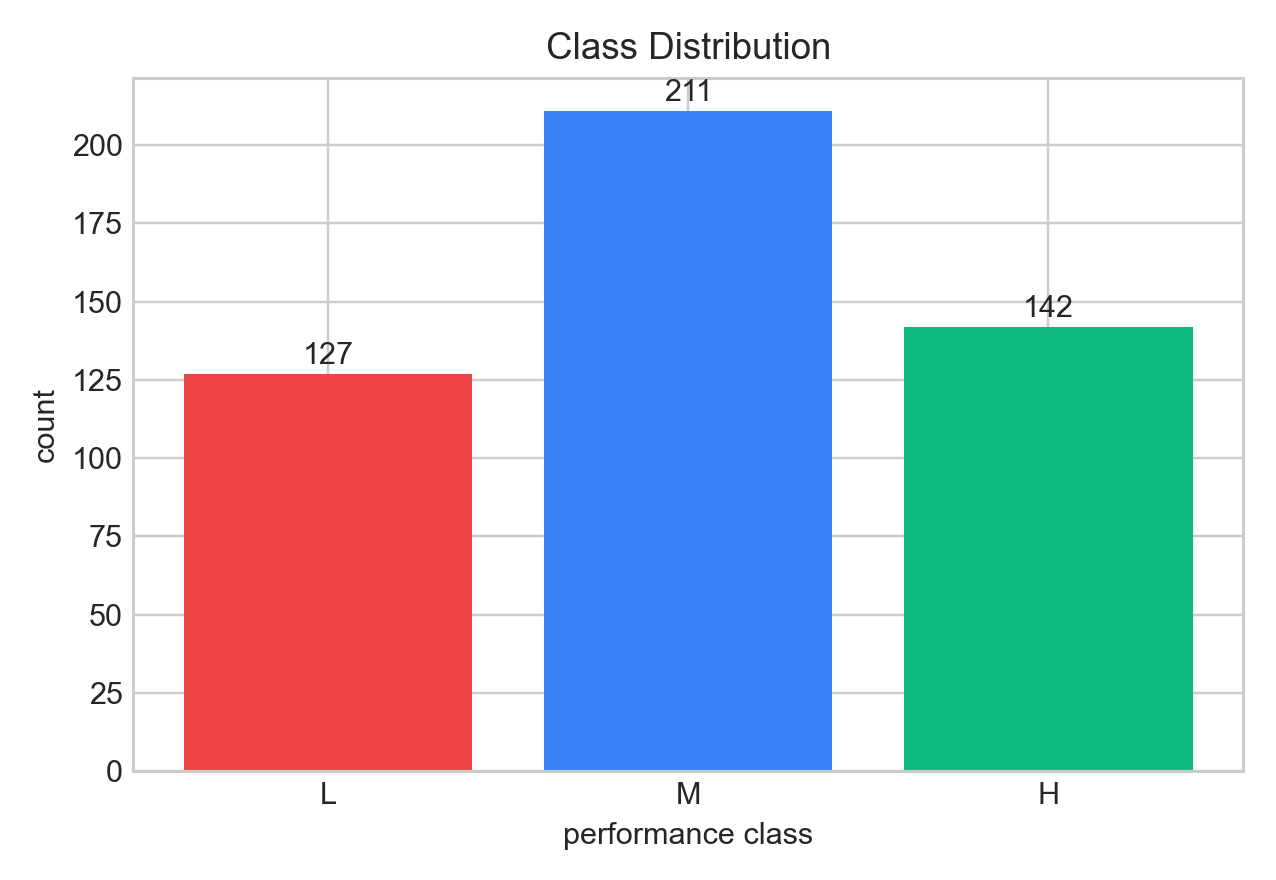
\includegraphics[width=0.68\linewidth]{figures/class_distribution.png}
    \caption{学生成绩等级类别分布}
    \label{fig:classdist}
\end{figure}

学习行为变量在不同成绩等级下的均值见表 \ref{tab:activity}。可以看出，高等级学生在举手、访问资源、查看公告和参与讨论四类行为上均明显高于低等级学生。例如，\texttt{H} 类学生平均访问课程资源次数为 78.75，而 \texttt{L} 类学生仅为 18.32。这说明学习活跃度与成绩等级之间存在较强联系。

\begin{table}[H]
\centering
\caption{不同成绩等级下主要学习行为均值}
\label{tab:activity}
\begin{tabular}{lrrrr}
\toprule
成绩等级 & 举手次数 & 访问资源 & 查看公告 & 参与讨论\\
\midrule
\texttt{L} & 16.89 & 18.32 & 15.57 & 30.83\\
\texttt{M} & 48.94 & 60.64 & 40.96 & 43.79\\
\texttt{H} & 70.29 & 78.75 & 53.38 & 53.66\\
\bottomrule
\end{tabular}
\end{table}

\begin{figure}[H]
    \centering
    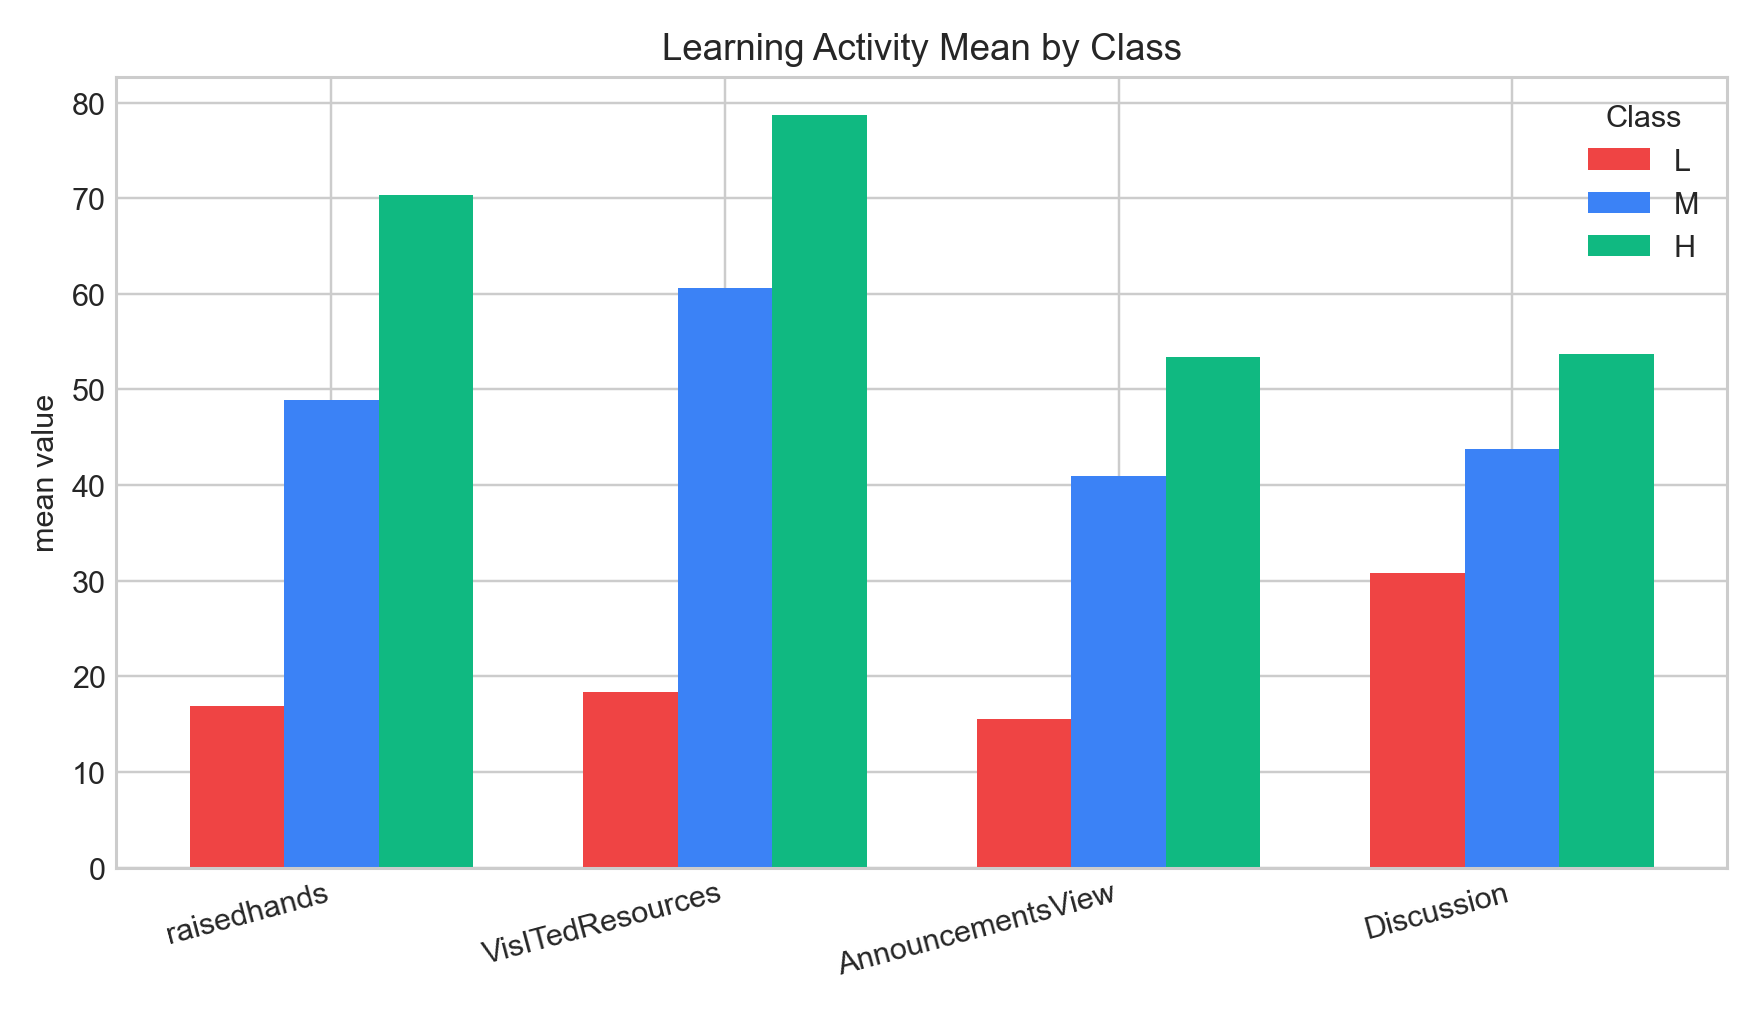
\includegraphics[width=0.9\linewidth]{figures/activity_mean_by_class.png}
    \caption{不同成绩等级下学习行为均值对比}
    \label{fig:activitymean}
\end{figure}

\subsection{算法实现}

实验程序使用 \texttt{pandas} 读取 CSV 数据，使用 \texttt{scikit-learn} 完成特征预处理、模型训练、交叉验证和模型评价。主要流程如下：

\begin{enumerate}
    \item 读取 \texttt{kalboard360\_xAPI\_Edu\_Data.csv}，确认数据规模、字段类型、缺失值和目标类别分布。
    \item 保存前 10 行数据、字段类型、缺失值统计、描述性统计、类别分布和不同成绩等级下的学习行为统计。
    \item 绘制目标类别分布图、学习行为均值图、学习行为箱线图和数值特征相关性热力图。
    \item 构造补充特征，包括 \texttt{activity\_total}、\texttt{activity\_mean}、\texttt{resource\_per\_raise}、\texttt{absence\_above\_7}、\texttt{parent\_answer\_yes}、\texttt{absence\_parent\_risk} 等。
    \item 将数据按 80\%/20\% 分层随机划分为训练集和测试集，其中训练集 384 条，测试集 96 条。
    \item 对类别特征使用 One-Hot 编码，对数值特征使用标准化处理。
    \item 分别训练 \texttt{Majority\_Baseline}、\texttt{LogisticRegression}、\texttt{SVM\_RBF}、\texttt{RandomForest} 和 \texttt{GradientBoosting} 五个模型。
    \item 在测试集上计算 Accuracy、Macro Precision、Macro Recall、Macro-F1 和 Balanced Accuracy，同时使用 5 折分层交叉验证估计模型稳定性。
    \item 对最佳模型保存混淆矩阵、分类报告和特征重要性图。
\end{enumerate}

完整 Python 程序见附录。

\section{实验结果与可扩展内容}

\subsection{实验结果}

图 \ref{fig:boxplot} 展示了四个学习行为变量在不同成绩等级下的箱线图。整体来看，\texttt{L} 类学生的举手次数和资源访问次数集中在较低区间，\texttt{H} 类学生明显更高，\texttt{M} 类学生位于二者之间。这说明学习行为数据可以为成绩等级分类提供有效信息。

\begin{figure}[H]
    \centering
    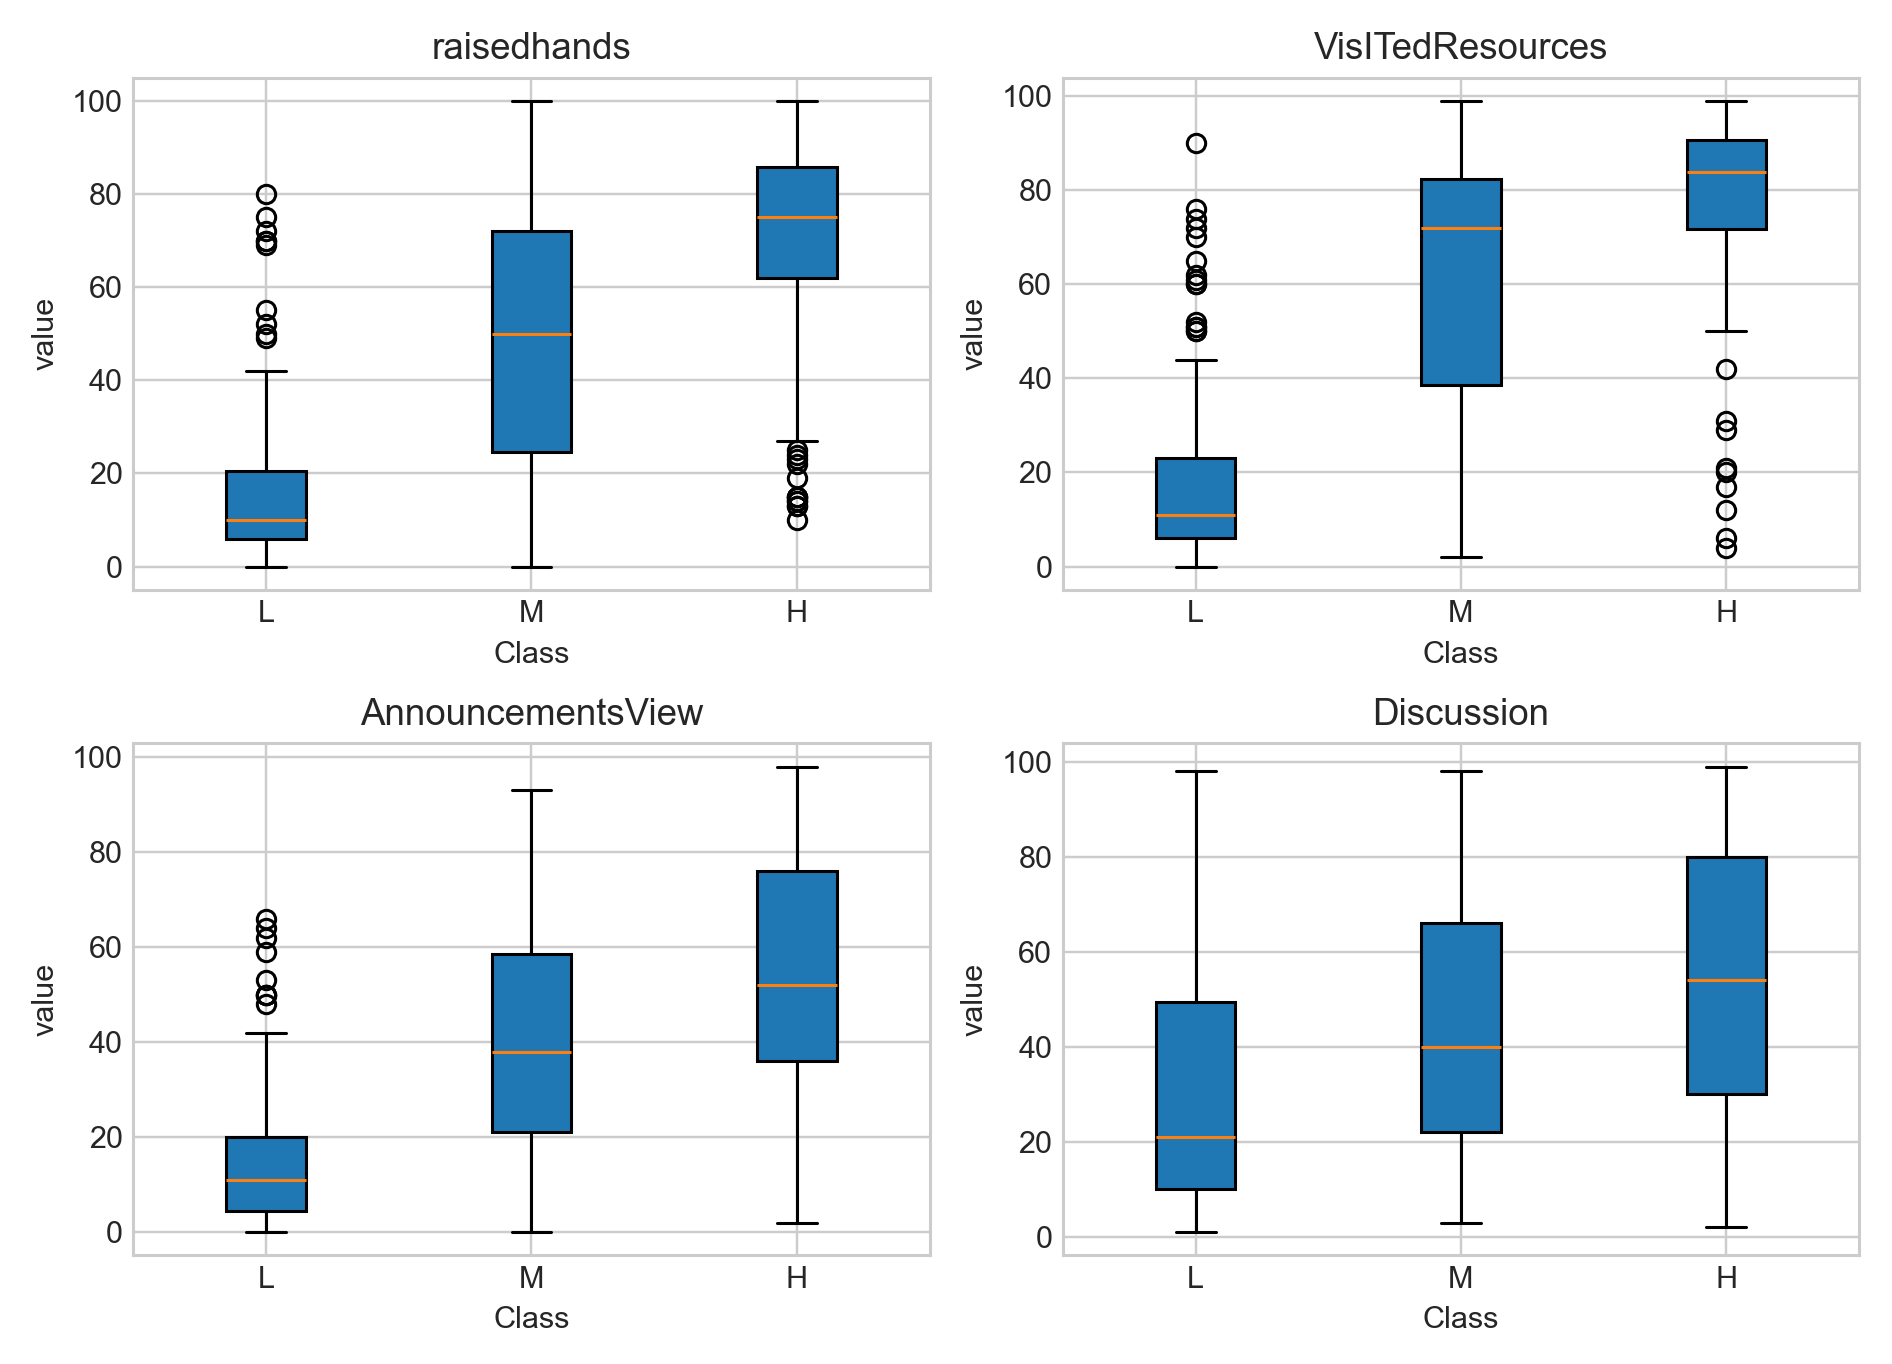
\includegraphics[width=0.9\linewidth]{figures/activity_boxplots_by_class.png}
    \caption{主要学习行为在不同成绩等级下的箱线图}
    \label{fig:boxplot}
\end{figure}

数值特征相关性热力图见图 \ref{fig:corr}。将目标等级映射为 \texttt{L}=0、\texttt{M}=1、\texttt{H}=2 后，可以看到 \texttt{raisedhands}、\texttt{VisITedResources}、\texttt{AnnouncementsView} 和 \texttt{Discussion} 与成绩等级整体呈正相关。其中，访问课程资源和举手次数的区分作用最明显。

\begin{figure}[H]
    \centering
    
\includegraphics[width=0.9\linewidth]{figures/correlation_heatmap.png}
    \caption{数值特征相关性热力图}
    \label{fig:corr}
\end{figure}

不同模型在测试集上的评价结果见表 \ref{tab:modelresult}。多数类基线模型只预测样本最多的 \texttt{M} 类，准确率为 0.4375，Macro-F1 仅为 0.2029，说明只依赖类别先验无法完成有效分类。加入学习行为、背景信息和家校互动特征后，所有机器学习模型均明显优于基线。

\begin{table}[H]
\centering
\caption{模型测试集评价结果}
\label{tab:modelresult}
\small
\begin{tabular}{lrrrrr}
\toprule
模型 & Acc. & Macro-P & Macro-R & Macro-F1 & Bal. Acc.\\
\midrule
\texttt{SVM\_RBF} & 0.8021 & 0.8066 & 0.8117 & 0.8090 & 0.8117\\
\texttt{RandomForest} & 0.7604 & 0.7665 & 0.7764 & 0.7707 & 0.7764\\
\texttt{GradientBoosting} & 0.7396 & 0.7455 & 0.7588 & 0.7513 & 0.7588\\
\texttt{LogisticRegression} & 0.7292 & 0.7298 & 0.7580 & 0.7385 & 0.7580\\
\texttt{Majority\_Baseline} & 0.4375 & 0.1458 & 0.3333 & 0.2029 & 0.3333\\
\bottomrule
\end{tabular}
\end{table}

从表中可以看到，\texttt{SVM\_RBF} 表现最好，测试集准确率为 0.8021，Macro-F1 为 0.8090，平衡准确率为 0.8117。随机森林次之，Macro-F1 为 0.7707。支持向量机优于树模型，说明该小样本数据中不同等级之间可能存在较复杂但相对平滑的非线性分类边界，RBF 核函数能够较好地捕捉这种边界。

\begin{figure}[H]
    \centering
    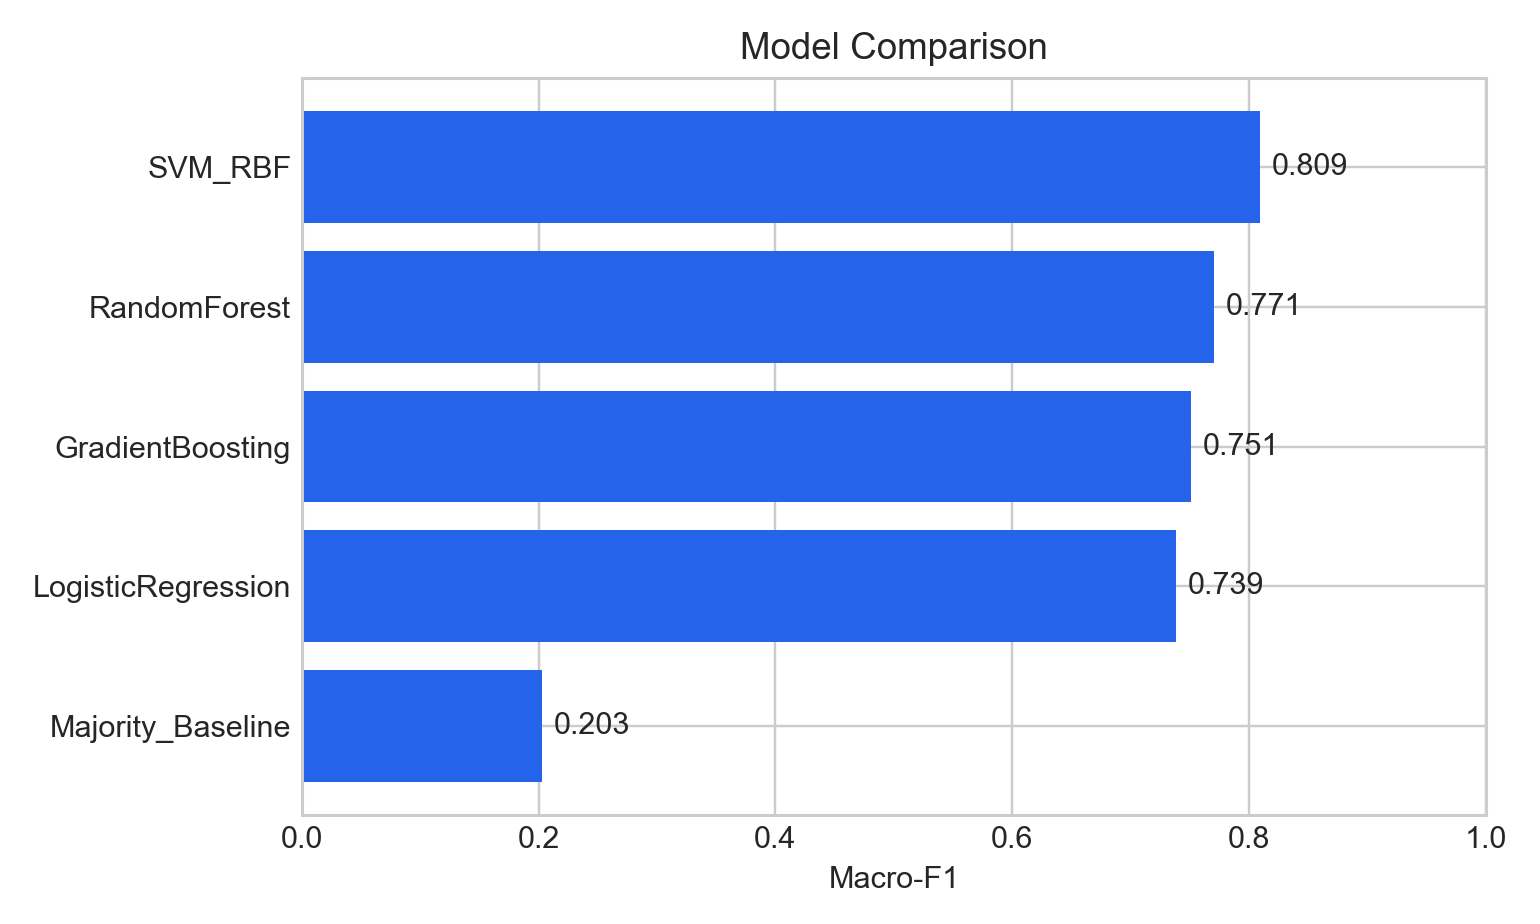
\includegraphics[width=0.78\linewidth]{figures/model_comparison_macro_f1.png}
    \caption{不同模型 Macro-F1 对比}
    \label{fig:modelcompare}
\end{figure}

表 \ref{tab:cvresult} 给出了 5 折分层交叉验证结果。交叉验证中 \texttt{SVM\_RBF} 的平均准确率为 0.7833，平均 Macro-F1 为 0.7902，平均平衡准确率为 0.7917，与测试集结果较接近，说明模型表现具有一定稳定性。随机森林的交叉验证 Macro-F1 为 0.7866，与 SVM 非常接近，也说明树模型同样是本任务中较可靠的选择。

\begin{table}[H]
\centering
\caption{模型 5 折分层交叉验证结果}
\label{tab:cvresult}
\begin{tabular}{lrrr}
\toprule
模型 & CV Accuracy & CV Macro-F1 & CV Balanced Acc.\\
\midrule
\texttt{SVM\_RBF} & 0.7833 & 0.7902 & 0.7917\\
\texttt{RandomForest} & 0.7792 & 0.7866 & 0.7876\\
\texttt{GradientBoosting} & 0.7417 & 0.7486 & 0.7465\\
\texttt{LogisticRegression} & 0.7250 & 0.7328 & 0.7444\\
\texttt{Majority\_Baseline} & 0.4396 & 0.2036 & 0.3333\\
\bottomrule
\end{tabular}
\end{table}

最佳模型 \texttt{SVM\_RBF} 的混淆矩阵见图 \ref{fig:cm}。测试集共有 96 条样本，其中 \texttt{L} 类 25 条、\texttt{M} 类 42 条、\texttt{H} 类 29 条。模型正确识别了 22 条 \texttt{L} 类、32 条 \texttt{M} 类和 23 条 \texttt{H} 类样本。主要错误发生在 \texttt{M} 类与相邻等级之间，这符合中间等级边界相对模糊的特点。

\begin{figure}[H]
    \centering
    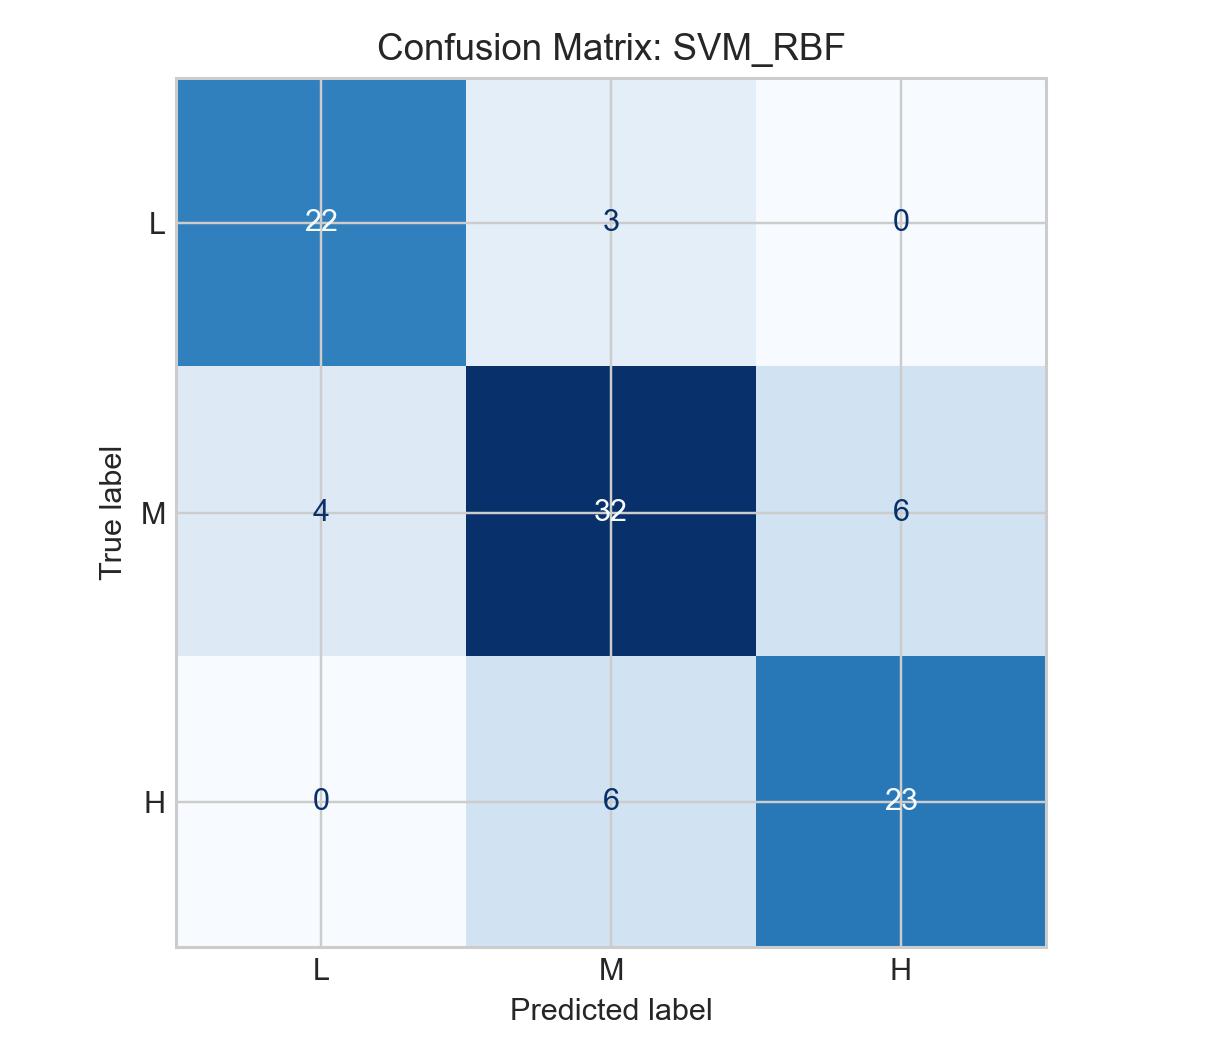
\includegraphics[width=0.62\linewidth]{figures/best_confusion_matrix.png}
    \caption{\texttt{SVM\_RBF} 测试集混淆矩阵}
    \label{fig:cm}
\end{figure}

从分类报告看，\texttt{L} 类的 F1 值为 0.8627，\texttt{M} 类的 F1 值为 0.7711，\texttt{H} 类的 F1 值为 0.7931。低等级学生识别效果最好，这对于实际教学预警具有一定意义，因为低成绩风险学生往往是最需要优先识别和干预的对象。

图 \ref{fig:importance} 给出了最佳模型的前 20 个特征重要性。由于 SVM 本身不直接提供树模型式的特征重要性，实验采用基于 Macro-F1 的置换重要性方法进行估计。结果显示，\texttt{absence\_above\_7}、\texttt{absence\_parent\_risk}、\texttt{VisITedResources}、\texttt{Discussion}、\texttt{relation\_mum} 和 \texttt{AnnouncementsView} 等特征位居前列，说明缺勤情况、家长参与和学习活动行为是影响分类结果的关键因素。

\begin{figure}[H]
    \centering
    
\includegraphics[width=0.9\linewidth]{figures/feature_importance_top20.png}
    \caption{最佳模型前 20 个重要特征}
    \label{fig:importance}
\end{figure}

\subsection{参数调优及可扩展内容}

本次实验采用固定参数完成模型比较。支持向量机使用 RBF 核函数，正则化参数 \texttt{C=6.0}，并设置 \texttt{class\_weight=balanced} 以缓解类别分布不均衡带来的影响。随机森林设置 500 棵树、最小叶节点样本数为 2，并使用类别平衡的子采样权重。后续若继续优化，可以从以下方向扩展：

\begin{itemize}
    \item 使用网格搜索或随机搜索进一步调节 SVM 的 \texttt{C} 和 \texttt{gamma}，寻找更合适的非线性分类边界。
    \item 对随机森林搜索 \texttt{max\_depth}、\texttt{min\_samples\_leaf} 和 \texttt{max\_features}，在拟合能力和泛化能力之间取得平衡。
    \item 使用更稳定的嵌套交叉验证估计最终泛化性能，减少单次训练测试划分带来的偶然性。
    \item 将 \texttt{Class} 看作有序等级，尝试有序分类或先回归后分箱的方法，利用 L、M、H 之间天然存在的顺序信息。
    \item 加入更细粒度的时间序列学习行为，例如最近一周资源访问变化、连续缺勤次数和作业提交趋势。
\end{itemize}

\section{讨论与结论}

\subsection{结果讨论}

通过实验可以得到以下结论。第一，学习行为特征与学生成绩等级关系明显。高等级学生在举手、资源访问、公告查看和讨论参与方面均显著高于低等级学生，其中 \texttt{H} 类学生平均资源访问次数为 78.75，而 \texttt{L} 类学生仅为 18.32。这说明在线学习平台记录的行为数据能够较好反映学生学习投入程度。

第二，缺勤和家校互动信息具有较高预测价值。置换重要性结果显示，\texttt{absence\_above\_7} 和 \texttt{absence\_parent\_risk} 位居前两位，说明缺勤超过 7 天会显著影响成绩等级判断；当缺勤较多且家长问卷未参与时，学生更可能处于风险状态。这一结果也符合教育场景中的常识。

第三，非线性模型整体优于线性模型。\texttt{SVM\_RBF} 的测试集 Macro-F1 达到 0.8090，高于逻辑回归的 0.7385；随机森林和梯度提升也优于逻辑回归。这说明学生成绩等级并不是由单一特征线性决定，而是由学习行为、缺勤、年级、科目和家庭支持等因素共同影响。

第四，中间等级 \texttt{M} 最容易发生混淆。混淆矩阵显示，\texttt{M} 类有一部分被误判为 \texttt{L} 或 \texttt{H}，这是因为中等表现学生本来就处于低高等级之间，行为特征可能同时具备两侧特征。实际应用时，可以将这类学生作为重点观察对象，而不只看模型给出的单一类别。

\subsection{结论总结}

本次实验完成了基于 Kalboard 360 学习管理系统数据的学生成绩等级分类任务。实验从 CSV 数据读取开始，依次完成数据预览、探索性分析、特征工程、类别编码、模型训练、交叉验证和结果可视化。结果表明，支持向量机 RBF 模型取得最佳测试集表现，准确率为 0.8021，Macro-F1 为 0.8090，平衡准确率为 0.8117；5 折交叉验证 Macro-F1 为 0.7902，说明模型具有一定泛化能力。

综合来看，学生成绩等级与学习活跃度、缺勤情况和家校互动密切相关。访问课程资源、参与讨论、查看公告和上课举手等行为越活跃，学生越可能处于较高成绩等级；缺勤较多且家长参与不足时，学生更容易出现低成绩风险。机器学习模型可以为教学预警提供辅助，但最终仍需要教师结合学生实际情况进行解释和干预。

\section{心得体会与思考}

\subsection{个人心得}

通过本次实验，我进一步理解了分类任务与前几次回归任务的差异。回归任务更关注数值误差大小，而分类任务除了整体准确率，还要关注每个类别是否都能被较好识别。对于本数据集，如果只看准确率，可能会忽略中间等级和低等级学生的识别情况；使用 Macro-F1 和混淆矩阵后，模型的优点和不足会更清楚。

本次实验也让我体会到，特征工程不只是机械地增加变量，而是要结合数据含义进行设计。例如，\texttt{absence\_parent\_risk} 将缺勤和家长问卷信息结合起来，反映了学生学习风险和家庭支持不足的叠加效应。这个特征在置换重要性中排名靠前，说明有业务含义的组合特征确实可能帮助模型。

\subsection{启发与思考}

本实验中的模型可以作为教学预警的初步工具，但不能直接替代教师判断。学生成绩受到很多因素影响，包括学习基础、家庭环境、课堂氛围、考试难度和心理状态等，而数据集中只包含学习平台记录的一部分信息。因此，模型预测为低等级并不意味着对学生能力的定性评价，而应被理解为“需要更多关注”的信号。

后续如果继续改进，我希望尝试两类方向：一是收集时间序列数据，观察学生学习行为随时间的变化，而不仅仅使用静态汇总特征；二是将模型输出从单一类别扩展为风险概率，让教师看到模型的不确定性。例如，当某名学生处于 \texttt{M} 和 \texttt{L} 的边界附近时，系统可以提示教师进一步查看其缺勤和资源访问情况，从而做出更细致的教学干预。

\section{附录}

\subsection*{算法代码及其注释}
\addcontentsline{toc}{subsection}{算法代码及其注释}

\VerbatimInput[breaklines,breakanywhere,fontsize=\small,frame=single,rulecolor=\color{gray!45}]{report_code.py}

\subsection*{关键运行结果汇总}
\addcontentsline{toc}{subsection}{关键运行结果汇总}

\begin{CodeBlock}
数据规模：(480, 17)
目标变量：Class，类别为 L/M/H
训练集样本数：384
测试集样本数：96

类别分布：
L：127
M：211
H：142

测试集模型结果：
SVM_RBF              Accuracy=0.8021, Macro-F1=0.8090, Balanced Accuracy=0.8117
RandomForest         Accuracy=0.7604, Macro-F1=0.7707, Balanced Accuracy=0.7764
GradientBoosting     Accuracy=0.7396, Macro-F1=0.7513, Balanced Accuracy=0.7588
LogisticRegression   Accuracy=0.7292, Macro-F1=0.7385, Balanced Accuracy=0.7580
Majority_Baseline    Accuracy=0.4375, Macro-F1=0.2029, Balanced Accuracy=0.3333

SVM_RBF 测试集分类报告：
L：precision=0.8462, recall=0.8800, f1-score=0.8627, support=25
M：precision=0.7805, recall=0.7619, f1-score=0.7711, support=42
H：precision=0.7931, recall=0.7931, f1-score=0.7931, support=29

最佳模型混淆矩阵：
       预测L  预测M  预测H
真实L    22     3     0
真实M     4    32     6
真实H     0     6    23

重要特征前五：
absence_above_7=0.0439
absence_parent_risk=0.0327
VisITedResources=0.0322
Discussion=0.0272
relation_mum=0.0252
\end{CodeBlock}

\end{document}
